\section{Introduction}
\label{section:p450/introduction}
The most common method of drug clearance among currently prescribed drugs is metabolism, which is the primary method of clearance for approximately 75\% of the top 200 most commonly prescribed drugs in the United States \cite{williams2004drug}.
\begin{figure}[h]
\centering
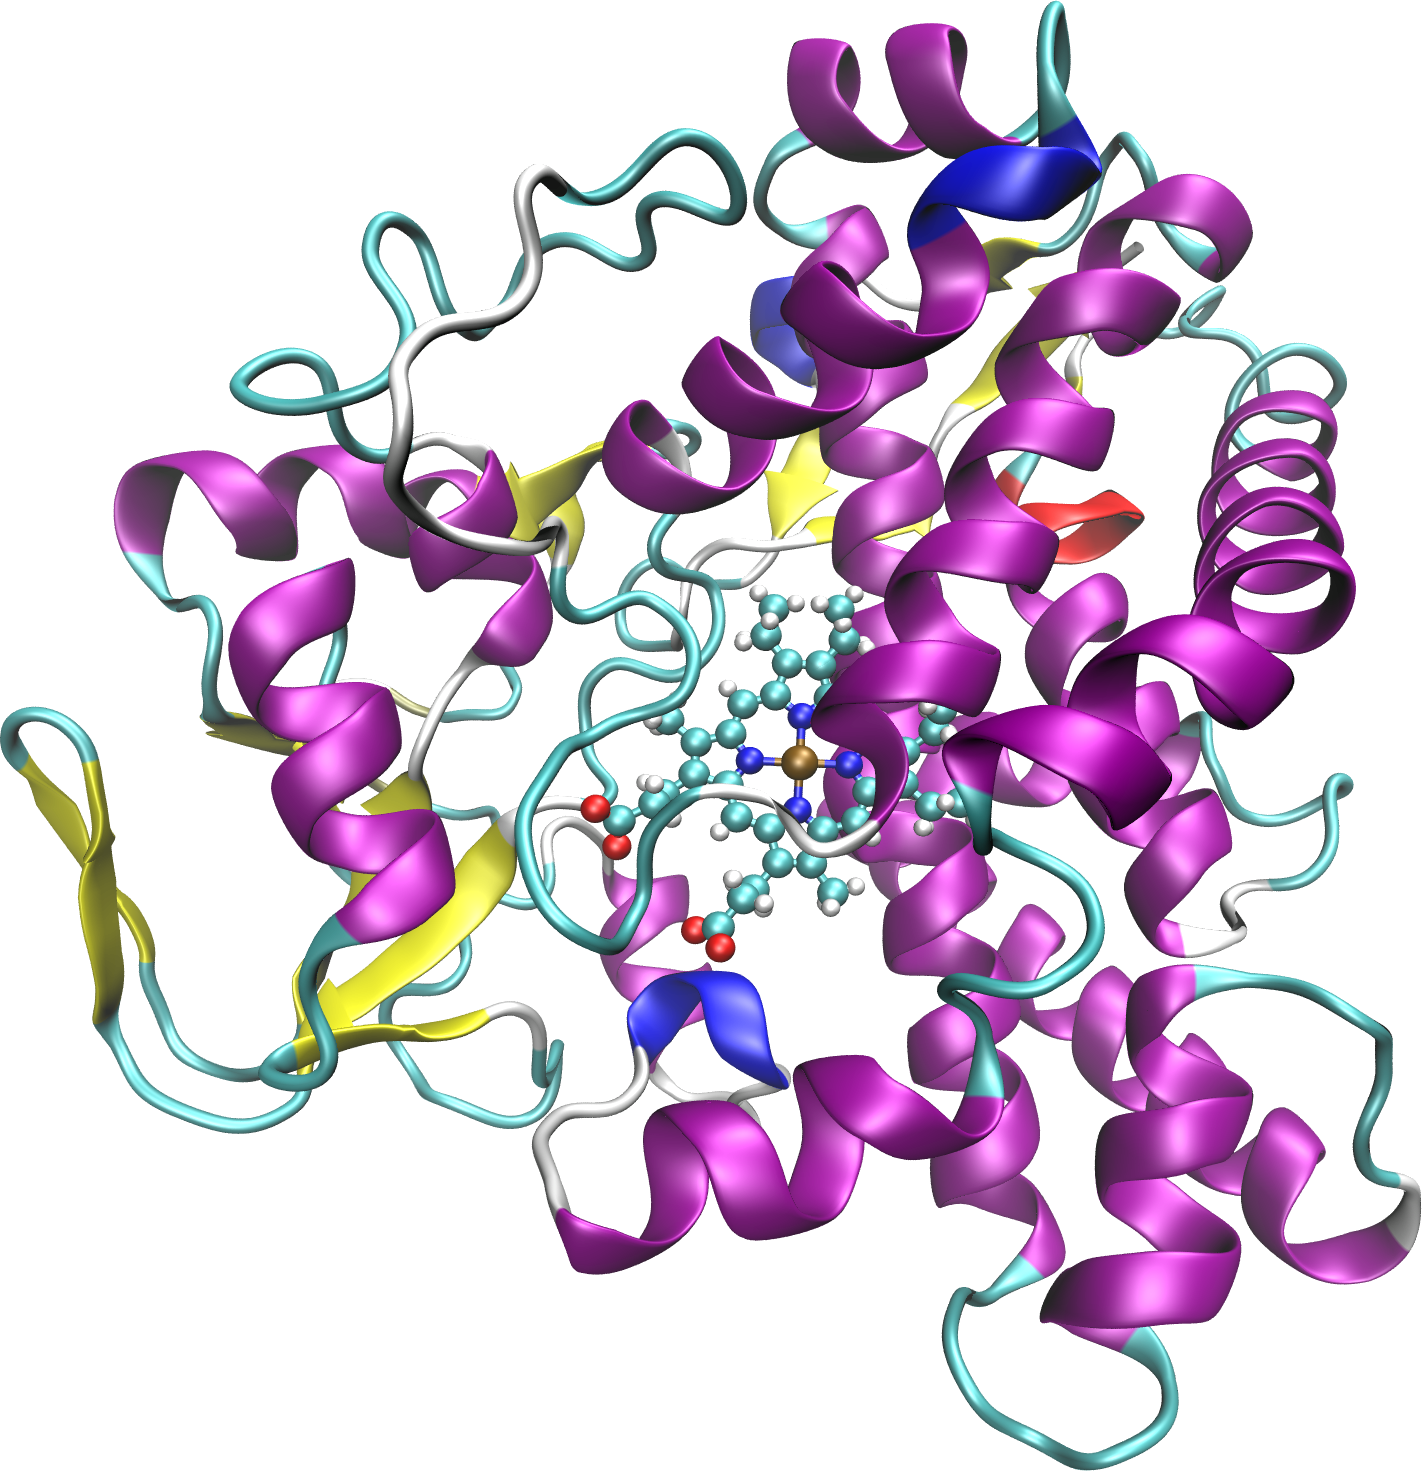
\includegraphics[width=0.5\textwidth]{figures/p450.png}
\caption{
The structure of cytochrome P450, taken from PDBid 1JFB, shown in cartoon representation.
The bonded heme group, shown as ball and stick model, is visible in the center.
The brown iron atom is chelated by four deep blue nitrogen atoms. 
}
\label{fig:p450}
\end{figure}
Cytochrome p450 is critical to drug metabolism, being active in approximately 75\% of drugs which are cleared in this method \cite{guengerich2007cytochrome}.
Of the human isoforms of P450, Cytochrome P450 2D6 (CYP2D6) is frequently involved metabolism of xenobiotics \cite{williams2004drug}, there are also high resolution crystal structures available for CYP2D6 \cite{rowland2006crystal} and thus it was used as a test case for this study.
As covered in \ref{subsubsection:lead_optimization}, accurately predicting  absorption, distribution, metabolism, and excretion, characteristics of drug compounds can be a critical determining factor in determining drug efficacy, performance in clinical development stages, and the overall costs of bringing new drugs to market.
Because of the ubiquity of P450 in metabolic reactions of drugs, there is no other single enzyme family as significant to determining ADME as P450.   

The general form of the reaction most frequently catalyzed by P450 is 
\begin{equation}
\mathrm{RH + O_{2} + NADPH + H^{+}> → ROH + H_{2}O + NADP^{+}}
\end{equation}


The specific locations of sites of metabolism (SOM) on small molecules can have a profound effect on the ADME characteristics of a small molecule.
Some cancer drugs such as epipodophyllotoxins, ifosphamide, tamoxifen, taxol and vinca alkaloids, are converted into their active states by oxygenation at specific locations by P450 \cite{kivisto1995role}.
P450 is the body's primary defense against toxicity, usually catalyzing the conversion of toxic compounds into harmless products \cite{gonzalez2005role,guengerich2001common}.
However in certain cases, such as acetaminophen, it is possible for P450 to convert a harmless reactant into a toxic product \cite{chen1998oxidation}, although usually these compounds would be eliminated during the clinical trial stages.
Additionally the different metabolites of a compound may be differentially cleared by the body having significant effects on bioavailability.
Because of the costs associated with testing ADME parameters in live organisms accurate computational predictions can significantly decrease both costs and times associated with drug development.

Because of its central role in drug metabolism P450 has already been a subject of a number of studies attempting to predict sites of metabolism and chemical metabolites \cite{afzelius2007state}.
A number of different classes of methods for predicting sites of metabolism by P450 have been developed.
Broadly speaking these can be classified into: quantitative structure-activity relationship (QSAR) based, pharmacophore-based, structure-based (docking), reactivity-based, and rule-based methods \cite{cruciani2005metasite}.
Rule based and pharmacophore based methods make predictions based on a subset of the drug structure, and it is possible for elements of the drug far from a possible site of metabolism to either prevent or promote metabolism at that location.
QSAR based approaches work best when the set of reactions being catalyzed are very similar, however P450 catalyzes a very broad range of reactions so these approaches are likewise somewhat limited in the case of P450.
Reactivity based methods are both very expensive to compute, being unsuited for screening a large database and do not take into account the structure of the P450 isoform \cite{singh2003model,chen1997oxidative,de2002factors}.
MetaSite, an approach which makes use of structural information of both the ligand and the P450 isoform process has achieved a 84.3\% prediction accuracy (296 of 351 total sites of metabolism correctly predicted), and the primary site of metabolism is identified in the top 3 ranked sites in over 90\% of cases \cite{cruciani2005metasite}.
However the sampling of P450 conformations done by MetaSite is quite limited, pre-computing a number of low energy conformations and then docking the substrate into each of those.

We have developed a similar approach which provides significantly more through sampling of the P450 substrate complex.
The new method, IDSite, makes use of the structures of both the P450 and the substrate as well as evaluating the intrinsic reactivity of the possible site of metabolism. 
